\documentclass{beamer}

\usepackage{beamerthemesplit}
%Kodierung festlegen, für UTF-8 Unterstützung entsprechend
\usepackage[utf8x]{inputenc}
% math. Symbole und Umgebungen
\usepackage{amsmath,amsfonts,amssymb}
% für Bilder
\usepackage{epsfig}
%\usecolortheme{crane} % Themes, die vor allem verschiedene Farblayouts besitzen
%\usefonttheme{professionalfonts} % Themes mit anderen Schriften
 
%\useoutertheme{infolines}  % oder: default | infolines | miniframes | shadow | sidebar | smoothbars |    smoothtree | split | tree
\usetheme{smoothbars} % komplett fertige Themes,
                    % oder auch: Hannover, PaloAlto, Hannover, Goettingen, Malmoe, CambridgeUS, Warsow ...
\useinnertheme{rounded} % vor allem Aussehen der Bulletts etc.



\title[kurzer Titel]{Kompletter Titel}
\author[Pascal Bernhard]{Pascal Bernhard}
\institute[BeLUG]{Berliner Linux User Group}
\date{5. Mai 2012}
\titlegraphic{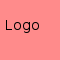
\includegraphics{logo}}
%\logo{\pgfimage{logo}}

\begin{document}
 


\frame{\titlepage}
 
%\section[Outline]{}
\frame{\tableofcontents}

\section{Introduction}
% in eckigen Klammern Kurzer Titel für Sidebar, in geschweiften Klammern kompletter Titel
\subsection[Overview]{Overview of existing methods}
%frame leitet einzelne Seiten einer Section / subsection ein
%frames können auch benannt werden
\begin{frame}
\frametitle{About existing methods}
 
\begin{figure}[\ht]

\includegraphics[scale=0.2]{testpic.png}
\end{figure}
 
% Stichpunkte können sehr schön in Blocks platziert werden
\begin{block}<2->{Different approaches:}
\begin{itemize}
\item<2-> first approach
\item<3-> Another approach
\item<4-> last approach
\end{itemize}
\end{block}
\end{frame}

\end{document}